\chapter{Opis projektnog zadatka}
		
		\textbf{\textit{dio 1. revizije}}\\
		
		\textit{Cilj projekta je razviti programsku podršku za stvaranje aplikacije „ParkShare“ koja će korisniku omogućiti da rezervira i plati parking. Korisnik će moći također pregledati sva slobodna parkirališna mjesta za automobile i bicikle. Prilikom pokretanja sustava korisnik će na mapi vidjeti obližnja parkirališta i dobit će rutu do najbližeg te će moći vidjeti ima li slobodnih mjesta kako ne bi došao na popunjeno parkiralište.
Neregistrirani korisnik šalje zahtjev za registraciju s odabranom ulogom koju želi, dakle voditelj parkinga ili klijent. Neregistriranom korisniku pokazuju se dostupa parkirališta i dostupna mjesta, a klijentima se prikazuje i zauzetost mjesta u stvarnom vremenu. Za registraciju korisniku su potrebni sljedeći podaci:
}
		\begin{packed_item}
			\item \textit{Korisničko ime }
			\item \textit{Lozinka }
			\item \textit{Ime }
			\item \textit{Prezime}
			\item \textit{Slika osobne }
			\item \textit{IBAN račun }
			\item \textit{Email adresa }
		\end{packed_item}
		
		\textit{Registracija završava potvrdom putem emaila korisnika, a voditelje mora potvrditi dodatno i administrator. Svaki korisnik aplikacije može vidjeti svoje privatne podatke u aplikaciji i može ih mijenjati. Također korisnik može izbrisati svoj korisnički račun. 
Postoje 3 vrste korisnika:
}
                \begin{packed_item}
			\item \textit{Klijent }
			\item \textit{Administrator }
			\item \textit{Voditelj parkirališta}
		\end{packed_item}

\textit{Administrator može vidjeti popis svih klijenata i voditelja i njihove osobne podatke i može ih mijenjati po volji ako je potrebno. Administrator može također pregledati sva parkirališta i njihova mjesta u aplikaciji i može mijenjati njihove podatke. Administrator može ukloniti ili promijeniti korisnički račun bilo kojeg ne-administrativnog korisnika. 
Voditelj zapisuje specifikacije svog parkirališta kao što su:
}
                \begin{packed_item}
			\item \textit{Naziv parkirališta }
			\item \textit{Opis }
			\item \textit{Fotografija}
                        \item \textit{Cjenik}
		\end{packed_item}

\textit{Voditelj ucrtava na karti svako parkirališno mjesto svog parkirališta i može za po želji odabrano parkirališno mjesto odrediti može li se rezervirati i postavlja senzore na parkirališna mjesta koji govore je li mjesto zauzeto. Nakon ucrtavanja parkirališnih mjesta zapisuje ukupan kapacitet parkirališta.
Klijent na karti pregledava parkirališta u svojoj blizini i klikom na njih može vidjeti dostupne informacije o tom parkiralištu ujedno i je li ima slobodnih mjesta na parkiralištu. Ukoliko klijent želi biti siguran, on može rezervirati parkirališno mjesto tako da upiše termin u kojem želi parkirališno mjesto i pokazat će mu sva dostupna parkirališna mjesta na karti koja se mogu rezervirati. Drugi način za rezervaciju je da klijent unaprijed odabere parkirališna mjesta koja želi i onda će mu se prikazati kalendar s dostupnim terminima rezervacije. Klijent može rezervirati mjesto na proizvoljno dugo vremena i može rezervacija biti definirana kao ponavljajuća. Voditelj za svoje parkiralište određuje cijenu ovisno o trajanju rezervacije. Ukoliko se klijent odluči rezervirati parkirališno mjesto, parking mu se odmah naplaćuje putem aplikacije, ako pak klijent dođe bez rezervacije i odabere slobodno parkirališno mjesto, parking se naplaćuje na licu mjesta. U aplikaciji svaki klijent posjeduje novčanik kojim plaća parking, a u svakom trenu može uplatiti određenu svotu novca u novčanik kako bi mogao plaćati parking.
Voditelji mogu vidjeti statistiku zauzetosti parkirališnih mjesta kroz vrijeme na svom parkiralištu. Prikupljaju se povijesne informacije kako je kroz vrijeme parkiralište bilo zauzeto i statistički se izračunava zauzetost u tom periodu vremena te se voditelju to prikazuje u obliku grafa. Voditelj može ucrtati najviše jedno parkiralište u aplikaciji, a parkirališna mjesta može ucrtavati i brisati kad god poželi, isto tako može izbrisati cijelo parkiralište. Voditelj parkinga može izmijeniti mogućnost rezervacije nekog parkirališnog mjesta te promijeniti cijenu parkinga. 
Napomenuli smo da će na svakom parkiralištu biti moguće ponuditi parking i biciklima. Voditelj parkirališta ne ucrtava parkirališna mjesta kao za automobile već samo određuje ukupan kapacitet parkirališta za bicikle. Korisnici bicikla neće morati brinuti o naplati parking jer se on neće naplaćivati takvim korisnicima samim tim neće imati ni opciju za rezervaciju parkinga. Svaki voditelj mora na karti naznačiti je li parkiralište dostupno i za bicikle kako bi korisnici znali na karti gdje mogu parkirati svoje bicikle. Parkirališna mjesta za bicikle neće imati senzor za očitavanje dostupnosti mjesta. U bazu podataka spremamo sve podatke o korisnicima i njihovim ovlastima. Pohranjujemo sve podatke o parkiralištima(ime, cijena, opis), također sve informacije o parkirališnim mjestima(zauzetost, tip). Svaki klijent u aplikaciji nakon korištenja određenog parkirališta dobiva „Like“ opciju, ikonu palčića gore  i dolje te odabire klikom je li mu se parkiralište sviđalo ili ne. Također može i zanemariti danu opciju nije obvezno odgovoriti. Aplikacija mora podržavati sustav u kojem može biti više korisnika odjednom.
}

		\eject
		
		\section{Primjeri u \LaTeX u}
		
		\textit{Ovo potpoglavlje izbrisati.}\\

		U nastavku se nalaze različiti primjeri kako koristiti osnovne funkcionalnosti \LaTeX a koje su potrebne za izradu dokumentacije. Za dodatnu pomoć obratiti se asistentu na projektu ili potražiti upute na sljedećim web sjedištima:
		\begin{itemize}
			\item Upute za izradu diplomskog rada u \LaTeX u - \url{https://www.fer.unizg.hr/_download/repository/LaTeX-upute.pdf}
			\item \LaTeX\ projekt - \url{https://www.latex-project.org/help/}
			\item StackExchange za Tex - \url{https://tex.stackexchange.com/}\\
		
		\end{itemize} 	


		
		\noindent \underbar{podcrtani tekst}, \textbf{podebljani tekst}, 	\textit{nagnuti tekst}\\
		\noindent \normalsize primjer \large primjer \Large primjer \LARGE {primjer} \huge {primjer} \Huge primjer \normalsize
				
		\begin{packed_item}
			
			\item  primjer
			\item  primjer
			\item  primjer
			\item[] \begin{packed_enum}
				\item primjer
				\item[] \begin{packed_enum}
					\item[1.a] primjer
					\item[b] primjer
				\end{packed_enum}
				\item primjer
			\end{packed_enum}
			
		\end{packed_item}
		
		\noindent primjer url-a: \url{https://www.fer.unizg.hr/predmet/proinz/projekt}
		
		\noindent posebni znakovi: \# \$ \% \& \{ \} \_ 
		$|$ $<$ $>$ 
		\^{} 
		\~{} 
		$\backslash$ 
		
		
		\begin{longtblr}[
			label=none,
			entry=none
			]{
				width = \textwidth,
				colspec={|X[8,l]|X[8, l]|X[16, l]|}, 
				rowhead = 1,
			} %definicija širine tablice, širine stupaca, poravnanje i broja redaka naslova tablice
			\hline \multicolumn{3}{|c|}{\textbf{naslov unutar tablice}}	 \\ \hline[3pt]
			\SetCell{LightGreen}IDKorisnik & INT	&  	Lorem ipsum dolor sit amet, consectetur adipiscing elit, sed do eiusmod  	\\ \hline
			korisnickoIme	& VARCHAR &   	\\ \hline 
			email & VARCHAR &   \\ \hline 
			ime & VARCHAR	&  		\\ \hline 
			\SetCell{LightBlue} primjer	& VARCHAR &   	\\ \hline 
		\end{longtblr}
		

		\begin{longtblr}[
				caption = {Naslov s referencom izvan tablice},
				entry = {Short Caption},
			]{
				width = \textwidth, 
				colspec = {|X[8,l]|X[8,l]|X[16,l]|}, 
				rowhead = 1,
			}
			\hline
			\SetCell{LightGreen}IDKorisnik & INT	&  	Lorem ipsum dolor sit amet, consectetur adipiscing elit, sed do eiusmod  	\\ \hline
			korisnickoIme	& VARCHAR &   	\\ \hline 
			email & VARCHAR &   \\ \hline 
			ime & VARCHAR	&  		\\ \hline 
			\SetCell{LightBlue} primjer	& VARCHAR &   	\\ \hline 
		\end{longtblr}
	


		
		
		%unos slike
		\begin{figure}[H]
			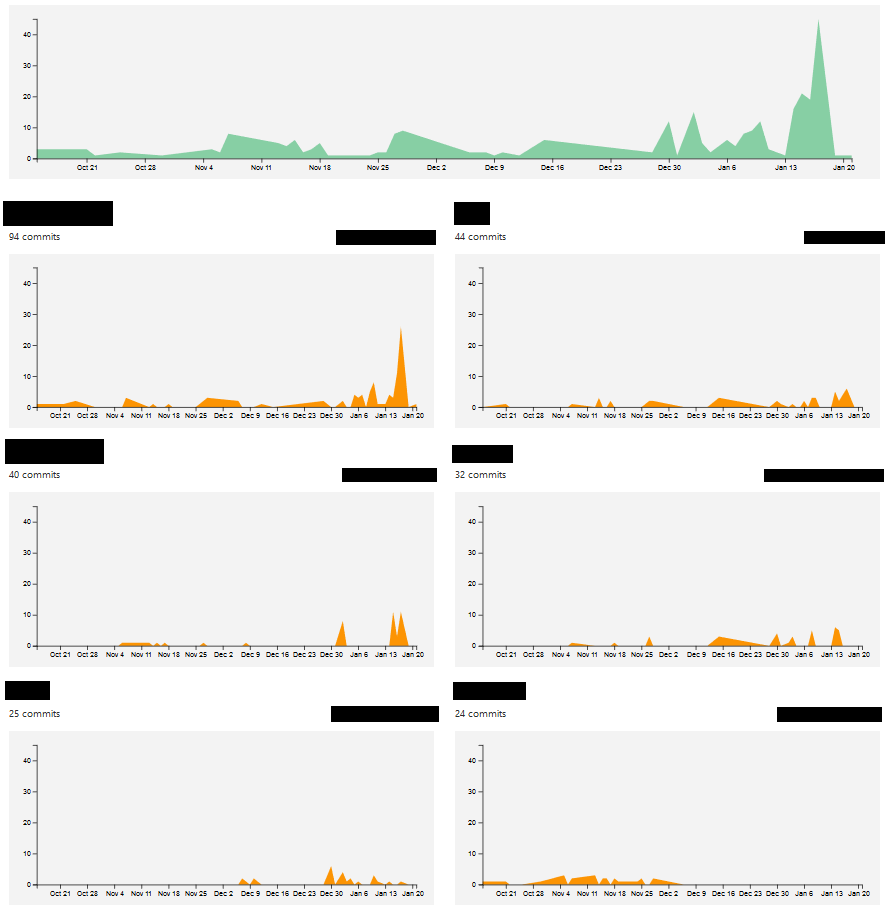
\includegraphics[scale=0.4]{slike/aktivnost.PNG} %veličina slike u odnosu na originalnu datoteku i pozicija slike
			\centering
			\caption{Primjer slike s potpisom}
			\label{fig:promjene}
		\end{figure}
		
		\begin{figure}[H]
			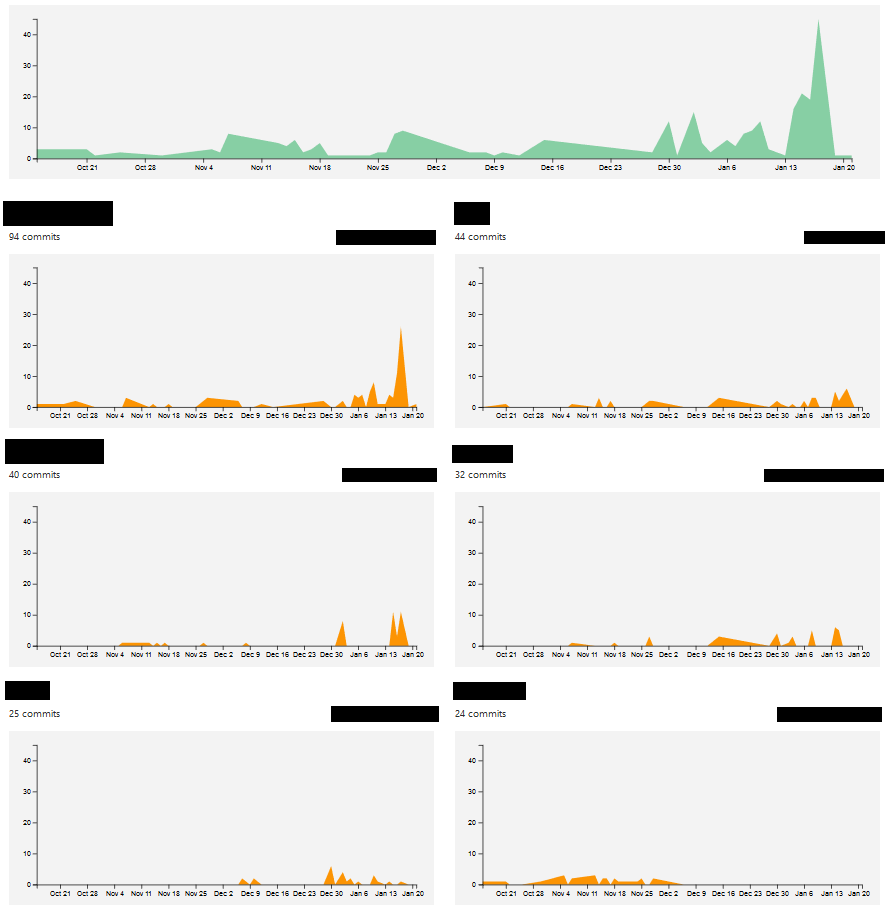
\includegraphics[width=\textwidth]{slike/aktivnost.PNG} %veličina u odnosu na širinu linije
			\caption{Primjer slike s potpisom 2}
			\label{fig:promjene2} %label mora biti drugaciji za svaku sliku
		\end{figure}
		
		Referenciranje slike \ref{fig:promjene2} u tekstu.
		
		\eject

		
